\documentclass[10pt,landscape]{article}
\usepackage{multicol,multirow}
\usepackage{calc}
\usepackage{ifthen}
\usepackage[landscape]{geometry}
\usepackage[colorlinks=true,citecolor=blue,linkcolor=blue]{hyperref}
\usepackage[fleqn]{amsmath}
\usepackage{amssymb,amsthm,amsfonts}
\usepackage{graphicx}
\usepackage{wrapfig}
\usepackage{cancel}
\usepackage[x11names]{xcolor}
\usepackage{framed}
\usepackage{array}

\ifthenelse{\lengthtest { \paperwidth = 11in}}
{ \geometry{top=.3in,left=.3in,right=.3in,bottom=.3in} }
{\ifthenelse{ \lengthtest{ \paperwidth = 297mm}}
{\geometry{top=1cm,left=1cm,right=1cm,bottom=1cm} }
{\geometry{top=1cm,left=1cm,right=1cm,bottom=1cm} }
}
\pagestyle{empty}
\makeatletter
\renewcommand{\section}{\@startsection{section}{1}{0mm}%
{-1ex plus -.5ex minus -.2ex}%
{0.5ex plus .2ex}%x
{\normalfont\large\bfseries}}
\renewcommand{\subsection}{\@startsection{subsection}{2}{0mm}%
{-1explus -.5ex minus -.2ex}%
{0.5ex plus .2ex}%
{\normalfont\normalsize\bfseries}}
\renewcommand{\subsubsection}{\@startsection{subsubsection}{3}{0mm}%
{-1ex plus -.5ex minus -.2ex}%
{1ex plus .2ex}%
{\normalfont\small\bfseries}}
\renewcommand{\arraystretch}{1.3}
\makeatother
\setcounter{secnumdepth}{0}
\setlength{\parindent}{0pt}
\setlength{\parskip}{0pt plus 0.5ex}
\setlength{\mathindent}{0pt}
\setlength{\columnseprule}{0.2pt}

\definecolor{shadecolor}{RGB}{200,240,240}
\definecolor{purple}{RGB}{128,0,128}
\definecolor{darkgreen}{RGB}{0,200,0}
\definecolor{darkorange}{HTML}{c2410c}

\renewcommand{\hrulefill}{\leavevmode\leaders\hrule height 0.2pt \hfill\kern0pt\relax}
\newcommand{\smallshade}[1]{{\setlength{\fboxsep}{0pt}\colorbox{shadecolor}{#1}}}

% -----------------------------------------------------------------------

\title{Numerical Analysis and Computer Algebra}

\begin{document}
    \raggedright
    \footnotesize

    \begin{center}
        \textbf{Numerical Analysis and Computer Algebra (Open Book)} \\
    \end{center}
    \begin{multicols}{3}
        \setlength{\premulticols}{1pt}
        \setlength{\postmulticols}{1pt}
        \setlength{\multicolsep}{1pt}
        \setlength{\columnsep}{2pt}

        \section{Newton Polynomial Interpolation}

For some interpolation problem (collocation), a polynomial 
$p(x) = c_0 + c_1x + c_2x^2 + \ldots + c_mx^m$
of degree $m$ is required such that the degree $m$ is minimal while meeting collocation conditions.

The data (measurements) are given by indexed pairs $(x_k,y_k)$ with $k=0,1,2,\ldots,n$.

\subsection{Aitken-Neville Recursion Formula}

Group together polynomials of a subset of the measurement into a global polynomial, e.g. for a dataset with three measurements:

\begin{align*}
	p_{0,1,2}(x)=\frac{(x-x_0)p_{1,2}(x) - (x-x_2)p_{0,1}(x)}{(x_2-x_0)}
\end{align*}

\subsection{Newton Basis Polynomials}

The basis polynomials with degree $k=0,1,2,\ldots,n$:

\begin{snugshade*}
	\begin{align*}
		\pi_0(x) & = 1 \\
		\pi_1(x) & = (x-x_0) \\ 
		\pi_2(x) & = (x-x_0)(x-x_1) \\
		\vdots \\
		\pi_n(x) & = (x-x_0)(x-x_1)\ldots(x-x_{n-1})
	\end{align*}
\end{snugshade*}

can be used to form a collocation polynomial using a linear combination 
$p(x)=a_0\pi_0(x) + a_1\pi_1(x) + \ldots + a_m\pi_m(x)$. 
This forms the system of linear equations
\begin{align*}
	y_0 & = a_0 \\
	y_1 & = a_0 + a_1(x_1-x_0) \\
	y_2 & = a_0 + a_1(x_1-x_0) + a_2(x_2-x_0)(x_2-x_1) \\
	\vdots \\
	y_n & = a_0+a_1\pi_1(x_n)+a_2\pi_2(x_n)+\ldots+a_n\pi_n(x_n)
\end{align*}

\emph{Stability}: Since the coefficient $a_k$ is determined by the first $k$ arguments,
we can extend the dataset with new data without altering existing coefficients.

\subsubsection{Divided Differences}

Due to stability, we can write the coefficients as $a_k(x_0,\ldots,x_k)$, only depending on the arguments lower than $k$.
Applying the Aitken-Neville formula, we receive for $k=0,1,\ldots,n$:

\begin{align*}
	y(x_0, x_2, \ldots, x_k)=\frac{y(x_1,x_2,\ldots,x_k) - y(x_0, x_1, \ldots, x_{k-1})}{(x_k - x_0)}
\end{align*}

\makebox[\columnwidth]{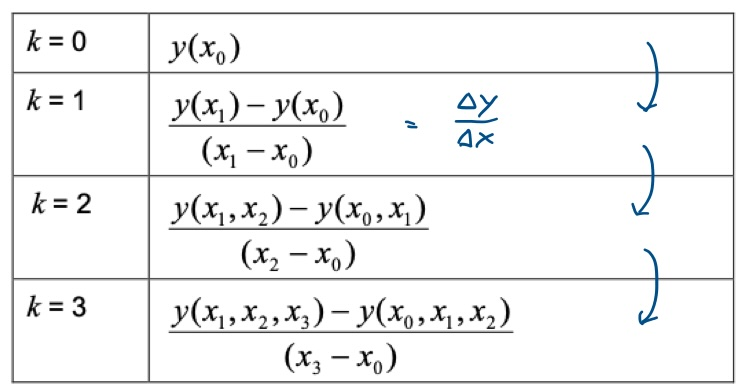
\includegraphics[width=0.6\columnwidth]{images/aitken-neville}}

\makebox[\columnwidth]{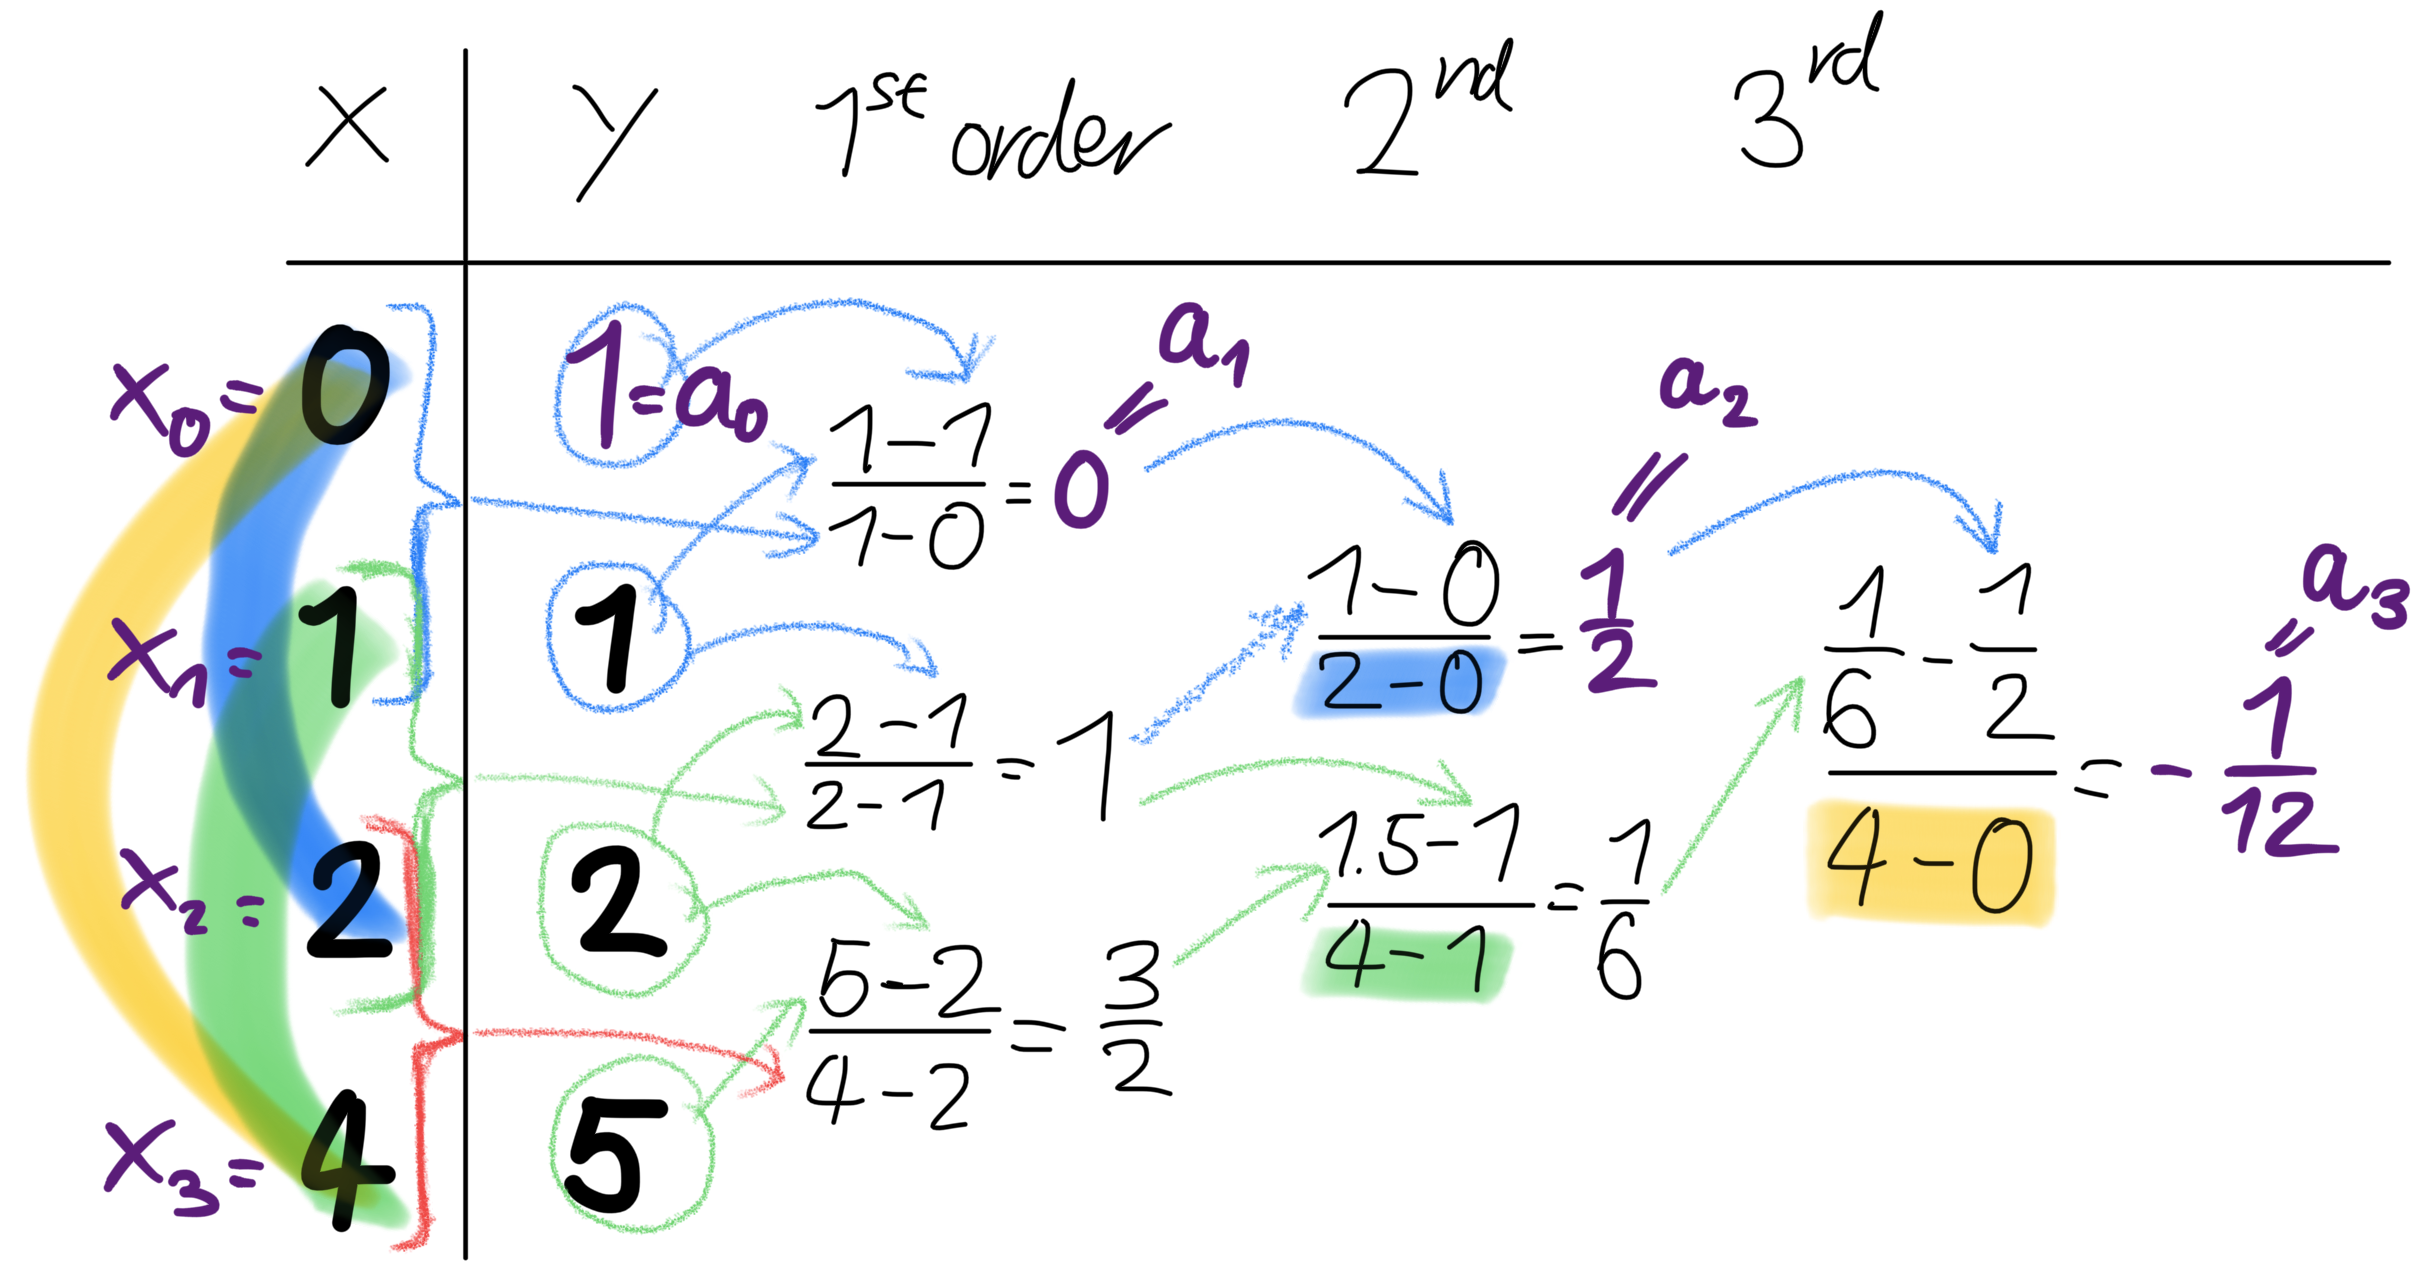
\includegraphics[width=0.6\columnwidth]{images/divided-differences}}


        \hrulefill
        \hspace{.5cm}

        \section{Hermite Interpolation}

Osculation or Hermite Interpolation is the collocation problem extended by the requirement to match
derivatives of model function at some of the arguments.

\subsection{Solving using Divided Differences}

We can use the property that a divided difference with repeated arguments can be interpreted as a derivative:

\begin{align*}
    \underbrace{y(x_0,\ldots,x_0)}_{(n+1)}=\lim_{\xi\to x_0}\frac{y^{(n)}(\xi)}{n!}=\frac{y^{(n)}(x_0)}{n!}
\end{align*}

For example:
\makebox[\columnwidth]{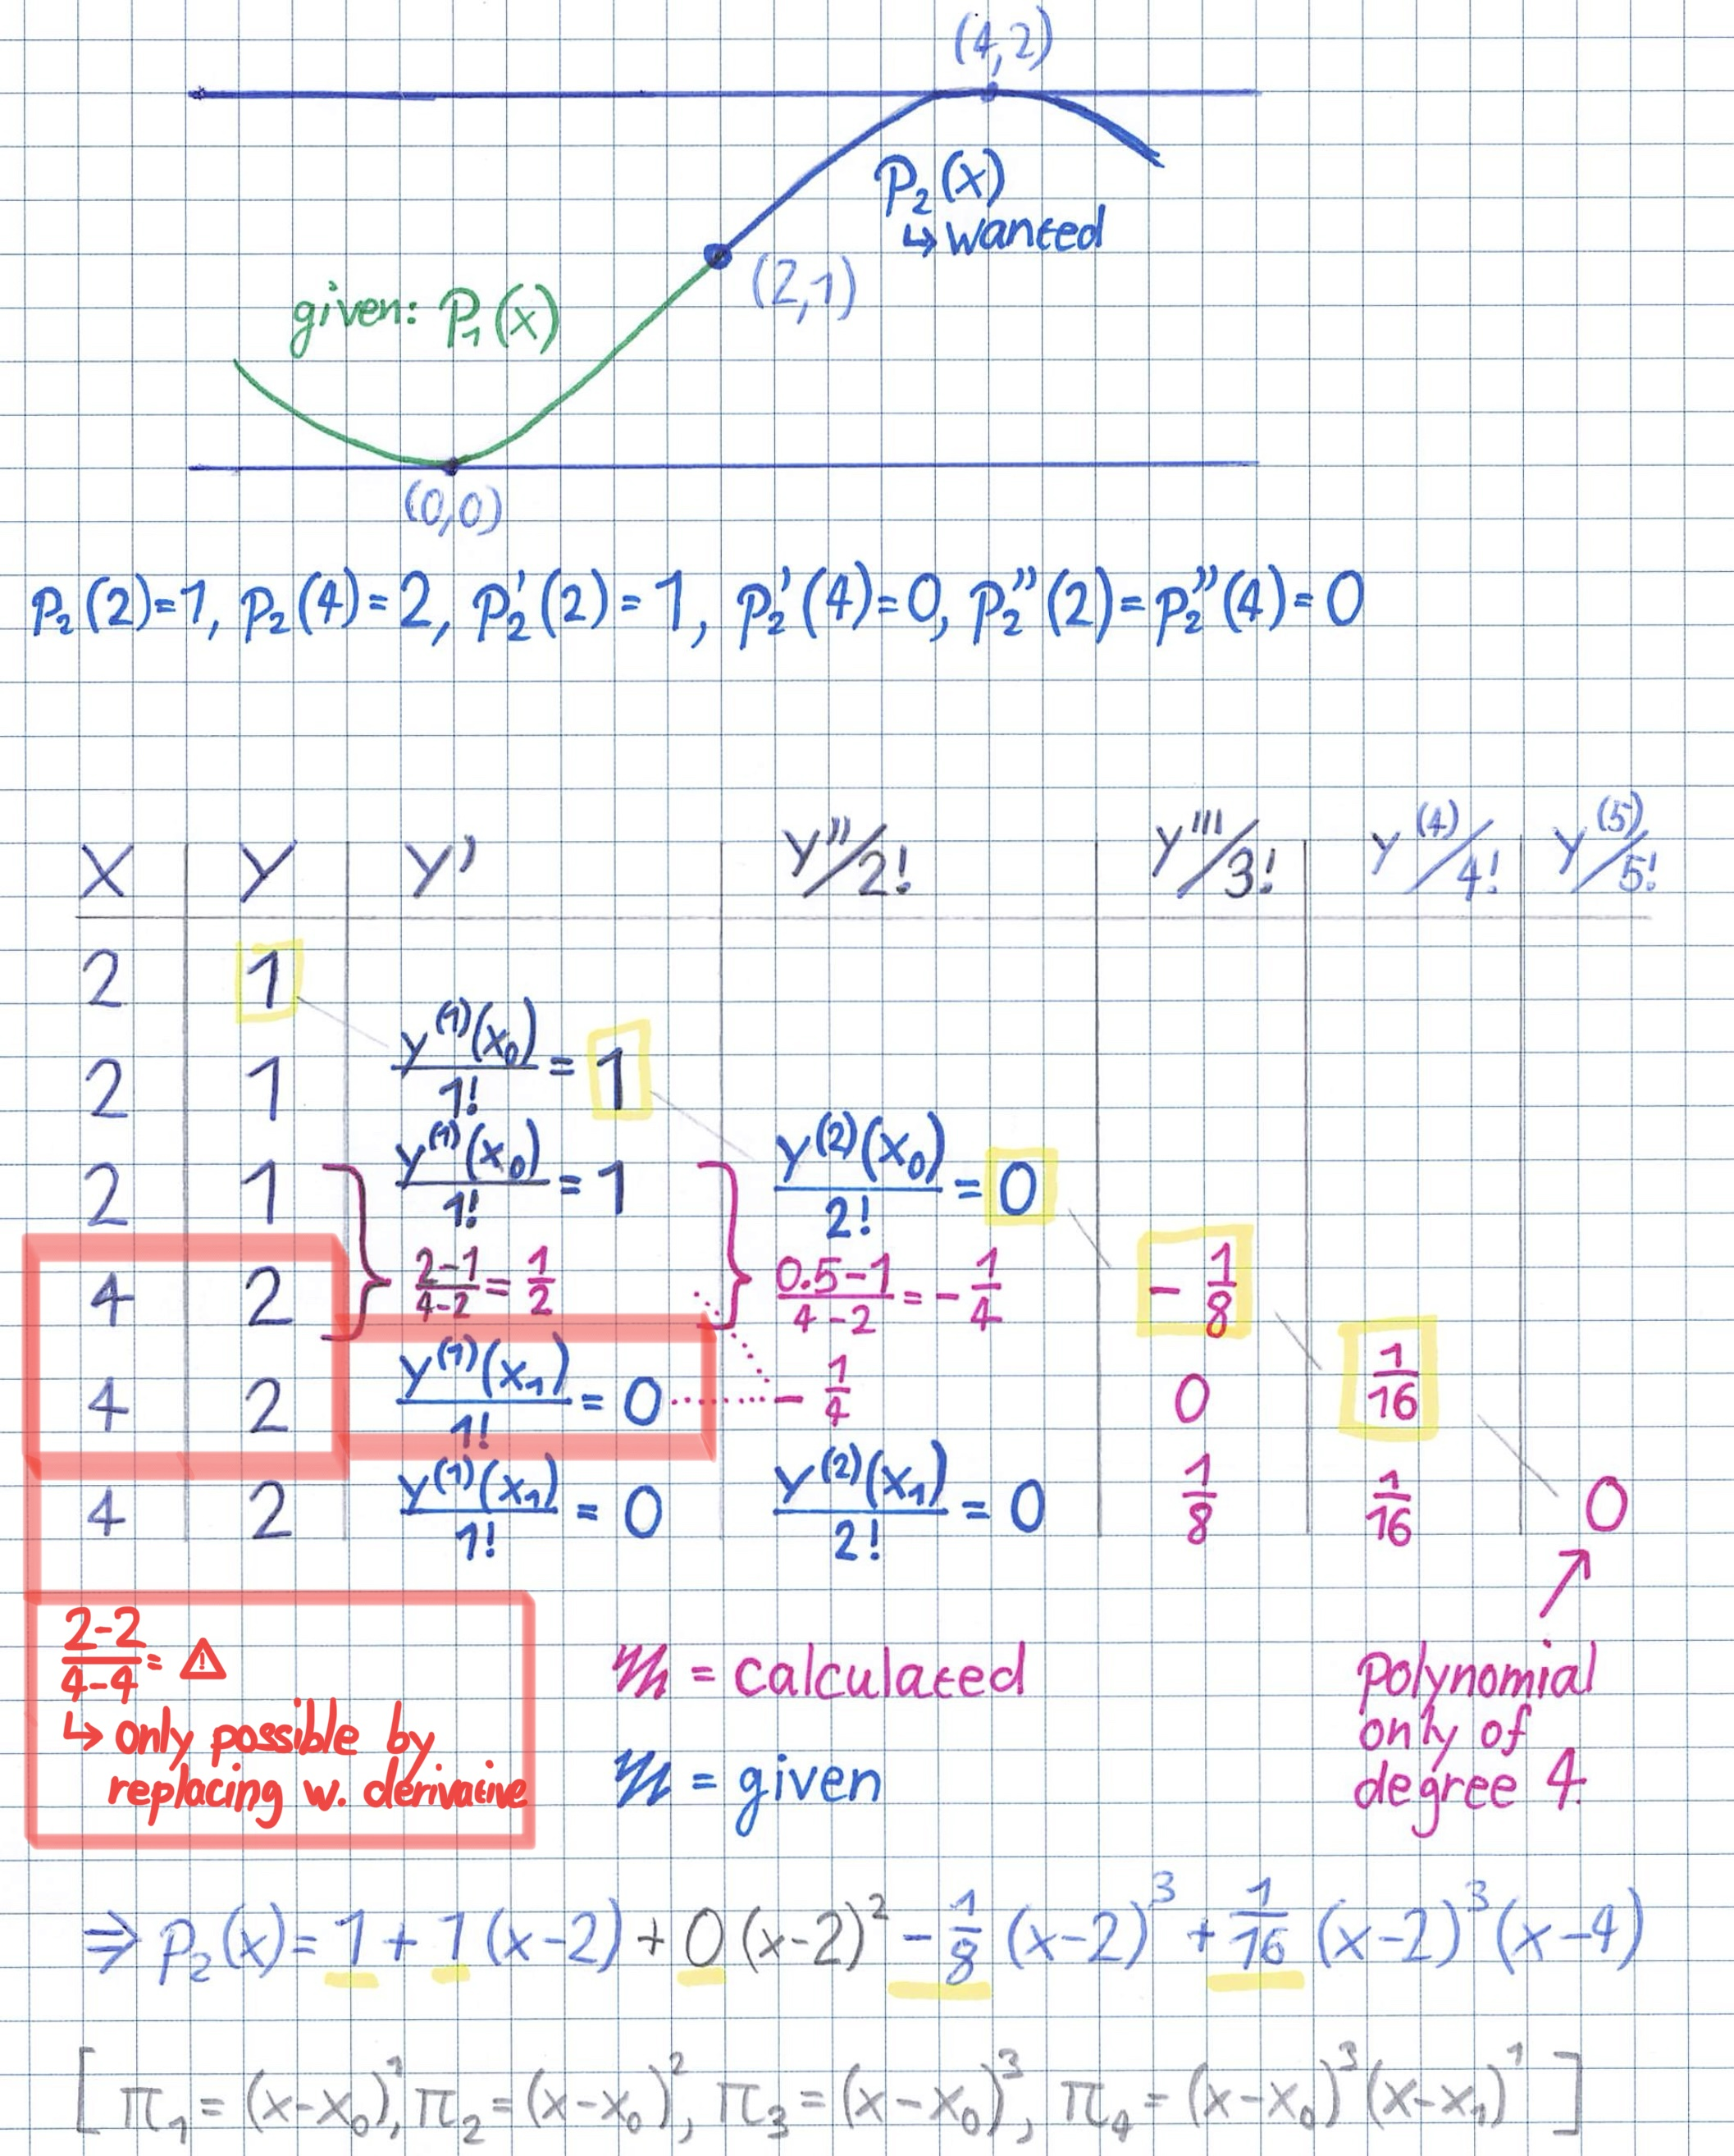
\includegraphics[width=\columnwidth]{images/hermite}}

$\pi_5$ would be $\pi_5 = (x-x_0)(x-x_0)(x-x_0)(x-x_1)(x-x_1)$ but the factor is zero, removing the need for it.

\subsection{Osculation Error Formula}

\begin{align*}
    \ & y(x)-p(x) = \frac{y^{(d)}(\xi)}{d!}(x-x_0)^{d_0}(x-x_1)^{d_1}\ldots(x-x_n)^{d_n} \\
    \ & x, \xi \in (\min x_i, \max x_i)_{i=0,1,\ldots,n}
\end{align*}

with $d$ denoting the total number of conditions and $d_i$ denoting the number of conditions for the argument $x_i\ (i=0,\ldots,n)$.
We have $d=d_0+d_1+\ldots+d_n$.

In the above example, this would be
\begin{align*}
    \frac{y^{(6)}(\xi)}{6!}(x-2)^3(x-4)^3
\end{align*}
($d$ = 6 constraints $\rightarrow$ at most degree of 5)


        \hrulefill
        \hspace{.5cm}

        \section{Multivariate Polynomial Interpolation}

\subsection{Bilinear Interpolation}

E.g.\ we want to interpolate color between four pixels.
We get the four basis functions $\{\pi_0(x), \pi_1(x)\} \times \{\pi_0(y), \pi_1(y)\}$
represented by a 2-fold tensor product:
\begin{align*}
    \overbrace{
        \left.
        \begin{bmatrix}
            1\cdot 1       & (x-x_0)\cdot 1 \\
            1\cdot (y-y_0) & (x-x_0)(y-y_0)
        \end{bmatrix}
        \right\}
    }^{\begin{matrix}
           \pi_0(x) & & & & \pi_1(x)
    \end{matrix}}
    \begin{matrix}
        \pi_0(y) \\
        \pi_1(y)
    \end{matrix}
\end{align*}

and the polynomial
\begin{align*}
    p(x,y) = &\ a_{0,0}\pi_0(x)\pi_0(y)
    + a_{1,0}\pi_1(x)\pi_0(y) \\
    \ & + a_{0,1}\pi_0(x)\pi_1(y)
    + a_{1,1}\pi_1(x)\pi_1(y)
\end{align*}

Then, the computation proceeds using divided differences in all steps:
\begin{enumerate}
    \item{
        Univariate interpolation for $x$ when holding $y=y_0$,
        ignoring a y parameter
        \begin{align*}
            p(x,y_0) = p(x_0,y_0)\pi_0(x) + \frac{p(x_n,y_0) - p(x_0, y_0)}{x_n - x_0}\pi_1(x)
        \end{align*}
        using the measurements at $x_0$ and $x_n$.
        We therefore receive a two-dimensional, univariate polynom
    }
    \item{
        Univariate interpolation for $x$ when holding $y=y_n$:
        \begin{align*}
            p(x,x_n) = p(x_0,y_n)\pi_0(x) + \frac{p(x_n,y_n) - p(x_0, y_n)}{x_n - x_0}\pi_1(x)
        \end{align*}
        giving a second polynomial ``at the other edge''
    }
    \item{
        Univariate interpolation for $y$:
        \begin{align*}
            p(x,y)=p(x,y_0)\pi_0(y)+\frac{p(x,y_1) - p(x,y_0)}{y_1-y_0}\pi_1(y)
        \end{align*}
        where we can substitute $p(x,y_1)$ and $p(x,y_0)$ with the above calculations
    }
\end{enumerate}


        \hrulefill
        \hspace{.5cm}

        \section{Spline Interpolation}

Given a set of measurement points with arguments $x_0,x_1,\ldots,x_n$.
($n$ = \# meas - 1)

\makebox[\columnwidth]{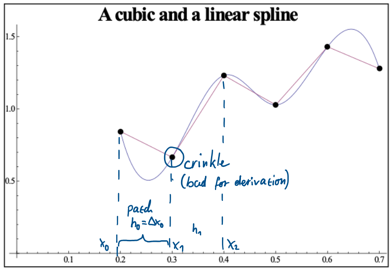
\includegraphics[width=0.6\columnwidth]{images/splines}}

The splines have to be a continuous curve ($C^0$) and often fulfill a smoothness condition
($C^1$ = cont. derivative, $C^2$ = cont. second derivative, ...).
Typical situation is that we seek patching polynomials of degree $d$ which must be a $C^{d-1}$ curve.
It is assumed that $n > d-1$ and gives a total of $n(d-1) + 2n - (d-1) = n(d+1) - (d-1)$ conditions.

\subsection{Cubic Splines}

For degree $d = 3$ and $i=0,1,\ldots,n-1$ we define a cubic polynomial
\begin{snugshade*}
    belonging to patch $[x_i,x_{i+1}]$ ($h=x_{i+1}-x_i = \Delta x_i$):
    \begin{align*}
        S_i(x) = a_i + b_i(x-x_i) + c_i(x-x_i)^2 + d_i(x-x_i)^3
    \end{align*}
\end{snugshade*}

To determine the coefficients, the following equations can be used:

\begin{snugshade*}
    \textbf{For $\mathbf{a_i}$:}
    \begin{align}
        \label{spline-a}
        a_i = y_i\ (i=0,\ldots,n-1)
    \end{align}
\end{snugshade*}
\begin{snugshade*}
    \textbf{For $\mathbf{b_i}$:}
    \begin{align}
        \label{spline-b}
        b_{i-1}=\frac{a_i-a_{i-1}}{h_{i-1}}-\frac{2c_{i-1}+c_i}{3}h_{i-1}\ (i=1,\ldots,n-1)
    \end{align}
    while the last one is
    \begin{align}
        \label{spline-bn}
        b_{n-1} = \frac{y_n - a_{n-1}}{h_{n-1}}-c_{n-1}h_{n-1}-d_{n-1}h_{n-1}^2
    \end{align}
\end{snugshade*}
\begin{snugshade*}
    \textbf{For $\mathbf{c_i}$ coefficients:} $((n-2)\times n)$ linear system
    (underdetermined $\Rightarrow$ many solutions)
    \begin{align*}
        \ & \resizebox{\columnwidth}{!}{$
        \begin{bmatrix}
            h_0 & 2(h_0 + h_1) & h_1          & 0       & \hdots               & 0       \\
            0   & h_1          & 2(h_1 + h_2) & h_2     & \hdots               & 0       \\
            0   & 0            & \ddots       & \ddots  & \ddots               & \vdots  \\
            0   & 0            & 0            & h_{n-3} & 2(h_{n-3} + h_{n-2}) & h_{n-2}
        \end{bmatrix}\cdot
        \begin{bmatrix}
            c_0    \\
            c_1    \\
            c_2    \\
            \vdots \\
            c_{n-1}
        \end{bmatrix}
        $} \\
        \ & =
        \begin{bmatrix}
            \vdots                                                                \\
            3\left(\frac{y_{i+1} - y_i}{h_i}-\frac{y_i - y_{i-1}}{h_{i-1}}\right) \\
            \vdots
        \end{bmatrix}_{i=1,\ldots,n-2}
    \end{align*}
\end{snugshade*}
\begin{snugshade*}
    \textbf{For $\mathbf{d_i}$:}
    \begin{align}
        \label{spline-d}
        d_{i-1} = \frac{c_i - c_{i-1}}{3h_{i-1}}
    \end{align}
\end{snugshade*}

\subsubsection{Natural Cubic Splines}
Fulfils the boundary condition $S''(x_0)=S''(x_n)=0$ and minimises the mean total curvature
$\int_{x_0}^{x_n}|f''(x)|^2\ dx$.
The tri-diagonal system of equations takes the regular form ($n-1$ equations for $n-1$ coeff.):
\begin{align*}
    \ & \resizebox{\columnwidth}{!}{$
    \begin{bmatrix}
        2(h_0 + h_1) & h_1          & 0       & \hdots               & 0                    \\
        h_1          & 2(h_1 + h_2) & h_2     & \hdots               & 0                    \\
        0            & 0            & \ddots  & \ddots               & \vdots               \\
        0            & 0            & h_{n-3} & 2(h_{n-3} + h_{n-2}) & h_{n-2}              \\
        0            & 0            & 0       & h_{n-2}              & 2(h_{n-2} + h_{n-1})
    \end{bmatrix}\cdot
    \begin{bmatrix}
        c_0     \\
        c_1     \\
        \vdots  \\
        c_{n-2} \\
        c_{n-1}
    \end{bmatrix}
    $} \\
    \ & =
    \begin{bmatrix}
        \vdots                                                                \\
        3\left(\frac{y_{i+1} - y_i}{h_i}-\frac{y_i - y_{i-1}}{h_{i-1}}\right) \\
        \vdots
    \end{bmatrix}_{i=1,\ldots,n-1}
\end{align*}

The $d$-coefficients take the form as described in (\ref{spline-d}) with
\begin{align}
    \label{spline-dn}
    d_{n-1} = -\frac{c_{n-1}}{3h_{n-1}}
\end{align}
and the $b$-coefficients as described in (\ref{spline-b}) and (\ref{spline-bn}).

\subsubsection{``Clamped''/Complete Cubic Splines}

These splines satisfy a first order derivative condition on the boundary arguments:
\begin{align*}
    S'(x_0)=y'_0\text{ and }S'(x_n)=y'_n
\end{align*}

The linear system for the $c$-coefficients:
\makebox[\columnwidth]{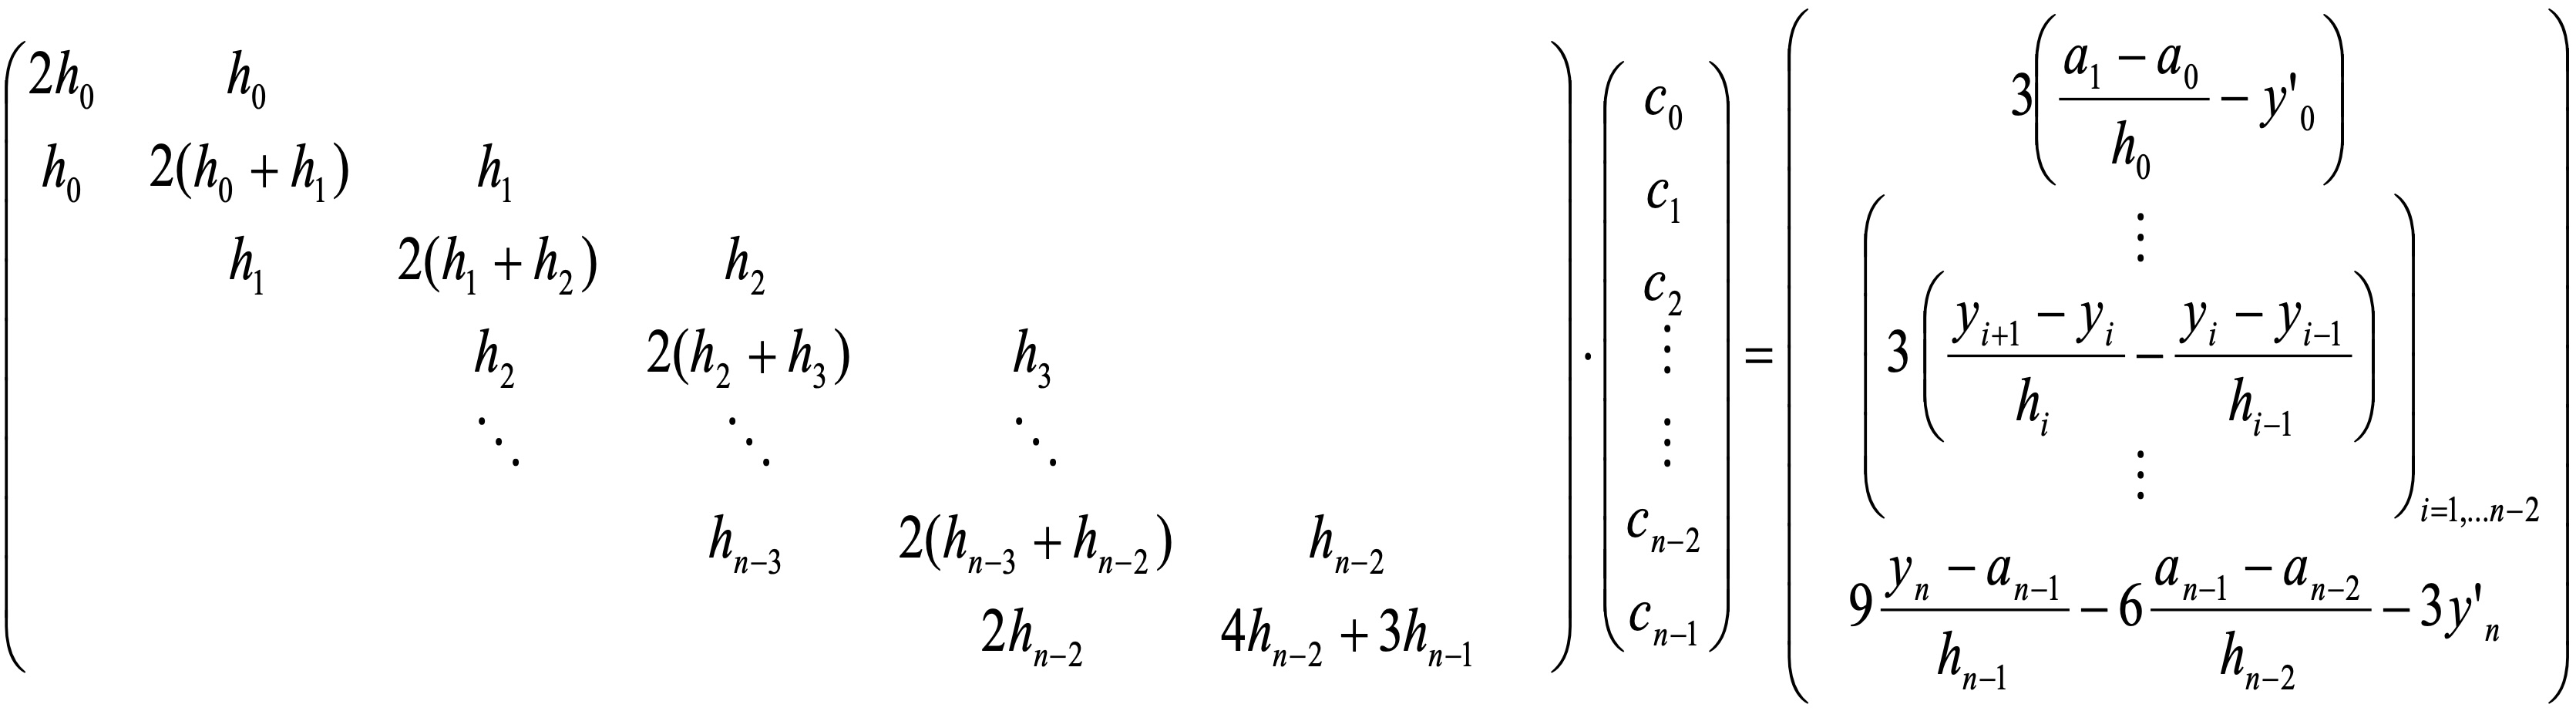
\includegraphics[width=\columnwidth]{images/clamped}}

From (\ref{spline-d}) we get $d_0,\ldots,d_{n-2}$,
from (\ref{spline-b}) we get $b_0,\ldots,b_{n-2}$ and $b_{n-1}$ from (\ref{spline-bn})
and finally $d_{n-1}$ from (\ref{spline-dn}).

\subsection{Error Formulas}
\begin{align*}
    |y(x)-S(x)| & \leq\max\frac{|y^{(4)}(x)|}{4!}\frac{5H^4}{16} = \max |y^{(4)}(x)|\frac{5}{384}H^4 \\
    |y'(x)-S'(x)| & \leq\max\frac{|y^{(4)}(x)|}{4!}H^3 = \max |y^{(4)}(x)|\frac{1}{24}H^3 \\
    |y''(x)-S''(x)| & \leq\max|y^{(4)}(x)|\frac{3}{8}H^2 \\
    & {\color{gray} x\in [x_0,x_n], H = \max_{i=0,\ldots,n-1}h_i}
\end{align*}

\subsection{Bernstein-B\'ezier Splines}

The basis functions for B\'ezier splines are the Bernstein polynomials:
\begin{snugshade*}
	\begin{align*}
		B_{i,n}(t) = \binom{n}{i}(1-t)^{n-i}t^i\ \ \ t\in[0,1]\ (i=0,1,\ldots,n)
	\end{align*}
\end{snugshade*}

by an affine transformation into the interval $[a,b]$ we get the transformed Bernstein polynomials:
\begin{align*}
	B_{i,n}(u,a,b) = B_{i,n}\left(\frac{u-a}{b-a}\right)
	= \frac{1}{(b-a)^n}\binom{n}{i}(b-u)^{n-i}(u-a)^i
\end{align*}
The polynomials have the following properties:
\begin{enumerate}
	\item They form a linear basis for the polynomials of order $n$
	\item $B_{i,n}(t)$ has exactly one maximum at $t = i\div n$
	\item $B_{i,n}(t)$ has a zero at 0 of order $i$ and a zero at 1 of order $n-i$
	\item Symmetry: $B_{i,n}(t) = B_{n-i,n}(1 - t)$
	\item They are a partition of unity: $\sum_{i=0}^n B_{i,n}(t) = 1$
\end{enumerate}

\paragraph{Bezier curves}
Using a set of $n+1$ $d$-dimensional control points (vectors) $\vec{P_0}, \vec{P_1}, \ldots, \vec{P_n}$ ($n\geq 2$) in $\mathbb{R}^d$:
\begin{snugshade*}
	\begin{align*}
		\vec{r}(t) = \sum_{i=0}^n \vec{P_i}B_{i,n}(t)\ \ \ t\in[0,1]
	\end{align*}
\end{snugshade*}
giving a spline of degree $n$.

The B\'ezier curve lies in the convex hull of its points:
$\{x\in R^{d}\mid x=\sum_{i=0}^{n}\lambda_{i}{\vec{P}}_{i}\wedge\sum_{i=0}^{n}\lambda_{i}=1\wedge 0\leq\lambda_{i}\leq1\}$
and has the following properites:
\begin{enumerate}
	\item The curve starts at point $\vec{P_0}$ and ends at point $\vec{P_n}$
	\item $\vec{r^{\prime}}(0) = n(\vec{P}_{1}-\vec{P}_{0}), \quad\vec{r^{\prime}}(1)=n(\vec{P}_{n}-\vec{P}_{n-1})$
	\item{
		$\vec{r^{''}}(0) = n(n-1)(\vec{P}_{2}-2\vec{P}_{1}+\vec{P}_{0})$,
		$\vec{r^{''}}(1)=n(n-1)(\vec{P}_{n}-2\vec{P}_{n-1}+\vec{P}_{n-2})$
		meaning that if we want to stop with no velocity, the last two points have to be the same
	}
	\item{
		$\frac{d}{d t^{k}}\vec{r}(0) = n(n-1)\cdots(n-k+1)\Delta^{k}\vec{P}_{0}$,
		$\frac{d}{d t^{k}}\vec{r}(1)=n(n-1)\cdots(n-k+1)\Delta^{k}\vec{P}_{n-k}$
	}
\end{enumerate}

\subsection{Casteljau Recursive Formula}
We can construct a B\'ezier curve similar to Aitken-Neville as a convex linear combination of points of lower order B\'ezier curves:
\begin{align*}
	\vec{r}_{\vec{p}_{0},\vec{p}_{1}\ldots\vec{p}_{n}}(t)
	= (1-t)\vec{r}_{\vec{p}_{0},\vec{p}_{1},\ldots\vec{p}_{n-1}}(t)+t\cdot\vec{r}_{\vec{p}_{1},\vec{p}_{2},\ldots\vec{p}_{n}}(t) \\
	t\in[0,1]
\end{align*}

\makebox[\columnwidth]{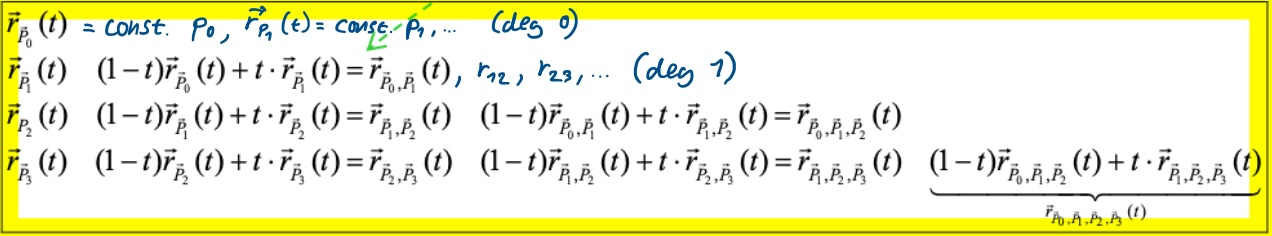
\includegraphics[width=\columnwidth]{images/casteljau}}


\subsection{Composite B\'ezier Curves}
Smush together multiple B\'ezier curves using common control points and smoothness conditions.
\\[1em]
\textbf{$\mathbf{C^1}$ smoothness condition:}
Given the curve $\vec{r}_p(t)$ using control points $\vec{P}_0,\ldots,\vec{P}_n$
and the curve $\vec{r}_q(t)$ using control points $\vec{Q}_0,\ldots,\vec{Q}_m$
and $\vec{P}_n=\vec{Q}_0$, then the composite curve is continuously differentiable at the common control point iff
\colorbox{shadecolor}{$\vec{r'}_p(1) = n(\vec{P}_n - \vec{P}_{n-1}) = m(\vec{Q}_1 - \vec{Q}_0) = \vec{r'}_q(0)$}.
\\[1em]
\textbf{$\mathbf{C^2}$ smoothness condition:}
\emph{Additionally to the conditions above},
for $C^2$ smoothness the two curves are only twice continuously differentiable at the common point iff
\begin{snugshade*}
	\begin{align*}
		\vec{r''}_p(1) & = n(n-1)\left(\vec{P}_n-2\vec{P}_{n-1}+\vec{P}_{n-2}\right) \\
		& = m(m-1)\left(\vec{Q}_2 - 2\vec{Q}_1 + \vec{Q}_0\right) = \vec{r''}_q(0)
	\end{align*}
\end{snugshade*}
\textbf{$\mathbf{C^k}$ smoothness condition:}
$j$ times continuously differentiable iff:
\begin{align*}
	\vec{r}^{(j)}_p(1) & = n(n-1)\cdots(n-j+1)(\Delta^{j}\vec{P}_{n-j}) \\
	& = m(m-1)\cdots(m-j+1)(\Delta^{j}\vec{Q}_{0}) = \vec{r}^{(j)}_q(0)
\end{align*}


        \hrulefill
        \hspace{.5cm}

        \section{Least-Squares Approximation}

\begin{itemize}
	\item Error = Residuum, errors = residuals. $e_i=r_i=y_i - \sum_{j=0}^ma_jg_j(x_i)$
	\item $\min_i\sum_i|e_i|$: $L^1$ norm
	\item $\min_i\sum_ie_i^2$: $L^2$ norm
	\item Basis functions $g_0,g_1,\ldots,g_m$ (m=degree, (polynom $x^m$))
	\item normalisation of data: $\frac{x-\mu}{\sigma}$ ($\mu$=mean, $\sigma$=deviation)
\end{itemize}

Some basis functions are:
\begin{itemize}
	\item{
		Trigonometric:
		\begin{align*}
			\left\{e^{i k x}\ |\ k\in Z\right\}{\text{or }}\left\{{\cos(k x){\mathrm{,}}\sin(k x)\ |\ k\in Z}\right\}\quad[x\in(0,2\pi)]
		\end{align*}
	}
	\item{
		Polynomials:
		\begin{align*}
			& \left\{x^{j}\ |\ j\in \mathbb{N}_{0}\right\} & \text{(standard monomials)} \\
			& \left\{\left({\frac{x-\mu}{\sigma}}\right)^{j}|\ j\in \mathbb{N}_{0}\right\} & \text{(normalised standard monomials)} \\
			& \left\{ \pi_{j}(x)\ |\ j\in \mathbb{N}_{0} \right\} & \text{(Newton polynomials)} \\
			& \left\{T_{j}(x)\ |\ j\in \mathbb{N}_{0}\right\} & \text{(Chebyshev, }x\in(-1,1))
		\end{align*}
		\begin{align*}
			& \left\{L_{j}(x)=\frac{e^{x}}{j!}\frac{d^{j}}{d x^{j}}\Big(e^{-x}x^{j}\Big)\ |\ j\in \mathbb{N}_{0}\right\}
			\text{(Laguerre, }x\in(0,\infty)) \\
			& \left\{H_{j}(x)=(-1)^{j}e^{\frac{x^{2}}{2}}\,{\frac{d^{j}}{d x^{j}}}\left(e^{-\frac{x^{2}}{2}}\right)\ |\ j\in \mathbb{N}_{0}\right\} \\
			&\quad\text{(Hermite, }x\in(0,\infty))
		\end{align*}
	}
	\item{
		Exponentials
		\begin{align*}
			\left\{ e^{\alpha kx}\ |\ k\in\mathbb{Z} \right\}
		\end{align*}
	}
\end{itemize}

\subsection{Design Matrix}
Given a \emph{measurement} $\{(x_i,y_i)\}_{i=0,\ldots,N}$ (with $x$ a vector in the multivariate case)
and a set of \emph{basis functions} $\{g_j\}_{j=0,\ldots,m}$,
the design matrix $G$ results from the linear system
$y_i=\sum_{j=0}^ma_jg_j(x_i)\quad(i=0,\ldots,N)$ with $N+1$ equations and $m+1$ unknowns:

\begin{snugshade*}
  \begin{align*}
    \underbrace{
      \begin{bmatrix}
        g_0(x_0) & \hdots & g_m(x_0) \\
        \vdots & \ddots & \vdots \\
        g_0(x_N) & \hdots & g_m(x_N)
      \end{bmatrix}
    }_{\text{Design matrix }G}
    \cdot
    \begin{bmatrix}
      a_0 \\
      \vdots \\
      a_m
    \end{bmatrix}
    =
    \begin{bmatrix}
      y_0 \\
      \vdots \\
      y_N
    \end{bmatrix}
  \end{align*}
\end{snugshade*}
that in general is overdetermined ($m<N$) thus the squared sum of residuals
$S=\sum_{i=0}^{N}\left(y_{i}-\sum_{j=0}^{m}a_{j}g_{j}(x_{i})\right)^{2}$
has to be minimised [$\downarrow$].

\paragraph{Normal Equation} Theorem: The squared sum of residuals $S$ is minimal iff:
\colorbox{shadecolor}{$
	G^T\cdot G\cdot a| = G^T\cdot y|\quad (a|\text{ and }y|\text{ are the column vectors})
$}

with $G^T\cdot G$ being a normal,
symmetric and relatively small $(m+1)\times(m+1)$ matrix resulting in $f(x)=\sum a_jg_j(x)$ as best $L^2$ fit for data.


        \hrulefill
        \hspace{.5cm}

        \section{Differentials \& Taylor-Formula}

The differential of a function at a specific input value $x_0$ is
$df(x_0) = f'(x_0)\ dx$ and has the rules
\begin{enumerate}
    \item \emph{Linearity:} $d(\alpha u \pm \beta v) = \alpha d(u)\pm \beta d(v)\quad(\alpha, \beta \in \mathbb{R})$
    \item \emph{Product:} $d(uv) = ud(v)+vd(u)$
    \item \emph{Quotient:} $d(u\div v) = (vd(u) - ud(v))\div v^2$
    \item \emph{Chain rule:} $d(v \circ u) = (v'\circ u)d(u)$
    \item \emph{Inversion:} $d(u^{-1}(y))=\frac{1}{u'(x)}dy\quad(x=u^{-1}(y))$
\end{enumerate}

\subsection{Univariate Taylor Formula}

If $y=f(x)$ is defined on the interval $I=[x0,x_0+h=x]$
\begin{align*}
    f(x_{0}+h) & =
    f(x_{0})+\frac{1}{1!} f^{(1)}(x_{0})h + \frac{1}{2!}f^{(2)}(x_{0})h^{2} + \cdots \\
    & + \frac{1}{n!}f^{(n)}(x_{0})h^{n}+R_{n}(x_{0},h)
\end{align*}

With the remainder error term $R_n(x_0, h)$:
\begin{itemize}
    \item{
        \emph{Lagrange form:}
        \begin{align*}
            \frac{h^{n+1}}{(n+1)!} f^{(n+1)}({\underbrace{x_{0}+\vartheta\cdot h}_{\xi}})
            \ \ {\color{gray} (\xi\in(x_{0},x_{0}+h),\ \vartheta\in(0,1)\,)}
        \end{align*}
    }
    \item{
        \emph{Cauchy form:}
        \begin{align*}
            \frac{h^{n}(1-\vartheta)^{n}}{n!}f^{(n+1)}(\underbrace{x_0+\vartheta\cdot h}_\xi)
            \ {\color{gray} (\xi\in(x_0,x_0+h), \vartheta\in(0,1))}
        \end{align*}
    }
\end{itemize}

\subsection{Multivariate Taylor Formula}

\begin{align*}
    f(\vec{x}_0 + \vec{h}) = &
    \overbrace{f(\vec{x}_0) + \frac{1}{1!}\vec\nabla f(\vec{x}_0)\cdot \vec{h}}^{\text{Linear approximation}} \\
    & + \underbrace{\sum_{|\alpha|=2}^N\frac{1}{\alpha!}\frac{\partial^{|\alpha|}f(\vec{x}_0)}{\partial x^\alpha}\vec{h}^\alpha}_{\text{Higher order deriv.}}
    + \underbrace{\sum_{|\alpha|=N+1}R_\alpha(\vec{x}_0,\vec{h})\vec{h}^\alpha}_{\text{Reminder term}}
\end{align*}

where the reminder terms are absolutely bounded by
$\displaystyle\max_{\vec{x}\in S}\left| \frac{1}{\alpha!}\frac{\partial^\alpha f(\vec{x})}{\partial x^\alpha} \right|$
with $|\alpha|=N+1$ and
$S={\vec{x}}_{0}+\left(\left[-h_{1},h_{1}\right]\times\left[-h_{2},h_{2}\right]\times\cdots\times\left[-h_{n},h_{n}\right]\right)$
is an $n$-dimensional ``rectangle'' at center $\vec{x}_0$.


\section{Jacobian}

For each vector-valued function
$\vec{f} : \mathbb{R}^n \mapsto \mathbb{R}^m : \vec{y} = \vec{f}(\vec{x}) = \left(f_1(\vec{x}),f_2(\vec{x}),\ldots,f_m(\vec{x})\right)$
we can find a Jacobian matrix with the rows being the gradients $\vec{\nabla}f_j$:
\begin{snugshade*}
    \begin{align*}
        J_f(\vec{x}) = \begin{bmatrix}
                           \frac{\partial f_1(\vec{x})}{\partial x_1} &
                           \frac{\partial f_1(\vec{x})}{\partial x_2} &
                           \ldots &
                           \frac{\partial f_1(\vec{x})}{\partial x_n} \\
                           \frac{\partial f_2(\vec{x})}{\partial x_1} &
                           \frac{\partial f_2(\vec{x})}{\partial x_2} &
                           \ldots &
                           \frac{\partial f_2(\vec{x})}{\partial x_n} \\
                           \vdots & \vdots & \ddots & \vdots \\
                           \frac{\partial f_m(\vec{x})}{\partial x_1} &
                           \frac{\partial f_m(\vec{x})}{\partial x_2} &
                           \ldots &
                           \frac{\partial f_m(\vec{x})}{\partial x_n}
        \end{bmatrix}_{\color{gray}m\times n}
    \end{align*}
\end{snugshade*}


in the case of the Jacobian matrix being a square matrix ($m=n$), it has a determinant $\det(J_f(\vec{x}))$.
The determinant of a linear transformation A (square matrix) allows the computation of ``transformed volumes'':
$\mathrm{vol}(A(C))=|\det(A)|\mathrm{vol}(C)$, meaning for $y_j = f_j(x_1,\ldots,x_n)\quad(j=1,...,m=n)$:
\begin{align*}
    \underbrace{dy_1dy_2\cdots dy_n}_\text{transformed volume element} = \det(J_f(\vec{x}))
    \underbrace{dx_1dx_2\cdots dx_n}_\text{volume element}
\end{align*}

\makebox[\columnwidth]{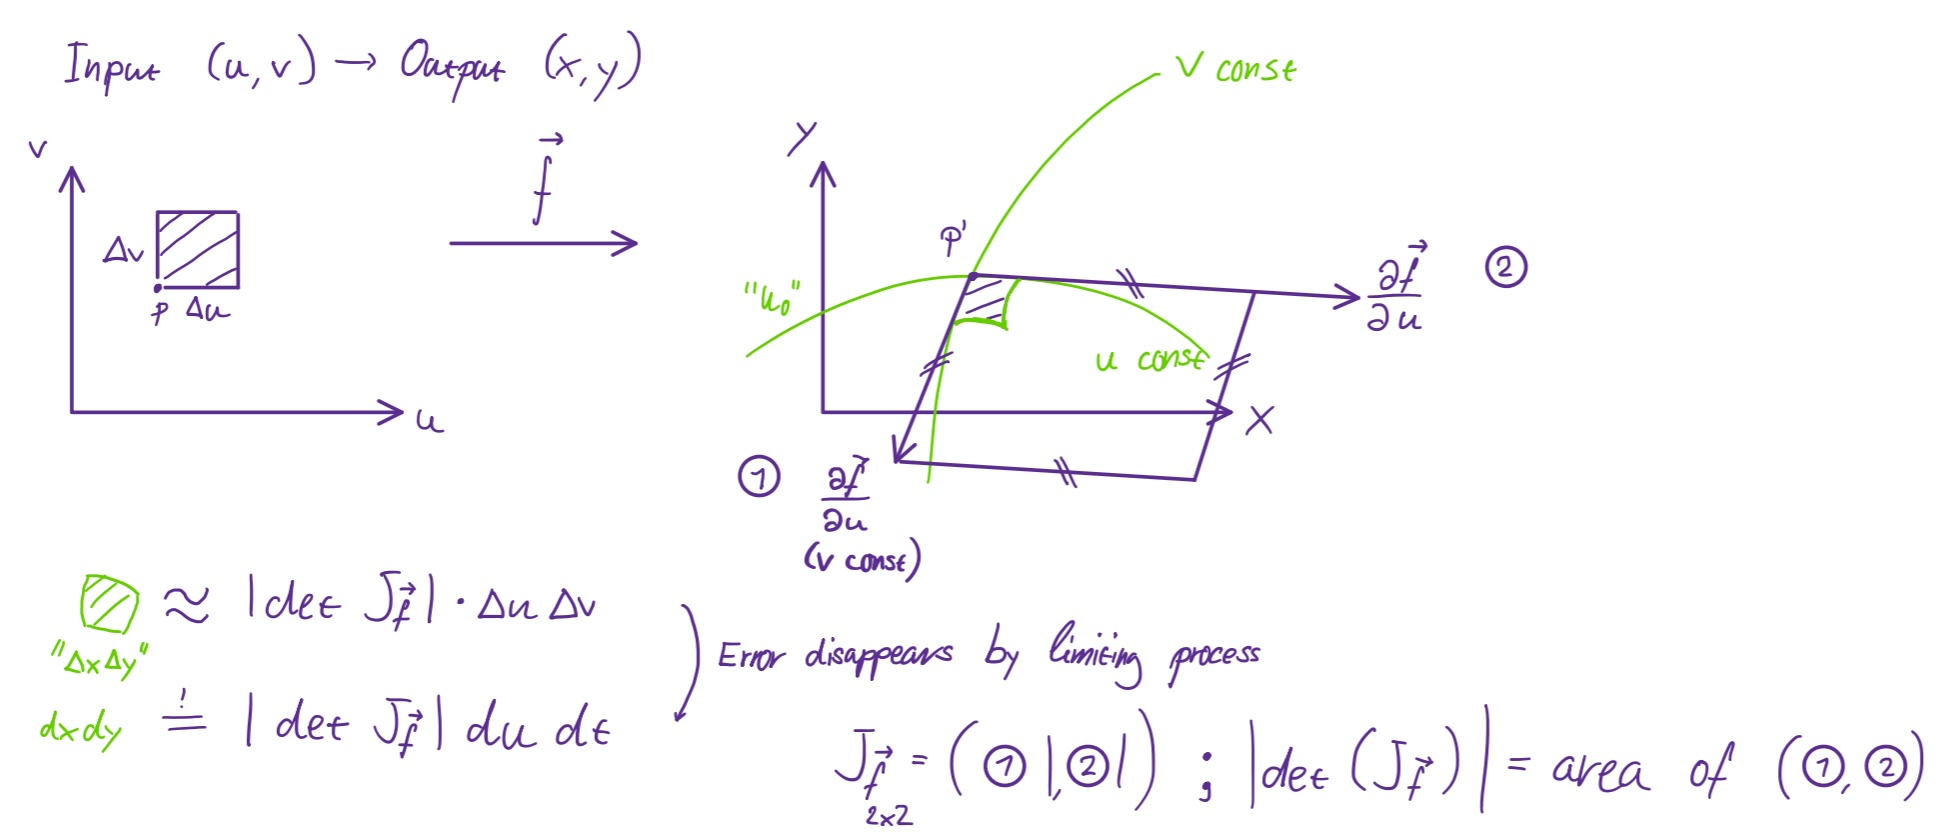
\includegraphics[width=\columnwidth]{images/jacobian}}

\textbf{For Example:} We want to compute the following integral on $\mathbb{R}^2$:
\begin{align*}
	\iint_{\mathbb{R}^2}e^{-\frac{x^2+y^2}{2}}\ dxdy
\end{align*}

by transformation to polar coordinates $(r,\varphi)$.
Hence, we have the transformation T: $(r,\varphi) \mapsto_T (x,y)$ with
\begin{align*}
	T(r,\varphi) = \begin{bmatrix}
		r\cos(\varphi) \\
		r\sin(\varphi)
	\end{bmatrix}
	=
	\begin{bmatrix}
		x(r, \varphi) \\
		y(r, \varphi)
	\end{bmatrix}
\end{align*}

and the Jacobian matrix:
\begin{align*}
	J_T =
	\begin{bmatrix}
		\frac{\partial x}{\partial r} & \frac{\partial x}{\partial \varphi} \\
		\frac{\partial x}{\partial r} & \frac{\partial x}{\partial \varphi}
	\end{bmatrix}
	=
	\begin{bmatrix}
		\cos(\varphi) & -r\sin(\varphi) \\
		\sin(\varphi) & r\cos(\varphi)
	\end{bmatrix}
\end{align*}

with the determinant $\det(J_T) = r\cos^2(\varphi) + r\sin^2(\varphi) = r$.
The transformed integral therefore looks like this:
\begin{align*}
	& \iint_{\mathbb{R}^2}e^{-\frac{x^2+y^2}{2}}\ dxdy \Rightarrow
	\int_0^{2\pi}\int_0^\infty e^{-\frac{\color{blue}r^2(\sin^2(\varphi)+\cos^2(\varphi))}{2}}{\color{purple}\det J_T}\ drd\varphi \\
	& = \int_0^{2\pi}\left(\int_0^\infty e^{-\frac{\color{blue}r^2}{2}}{\color{purple}r}\ dr\right)d\varphi 
	= \int_0^{2\pi} \left[ -e^{-\frac{r^2}{2}} \right]^\infty_0\ d\varphi \\
	& = \int_0^{2\pi} 1\ d\varphi = [\varphi]^{2\pi}_0 = 2\pi
\end{align*}


        \hrulefill
        \hspace{.5cm}

        \section{Numerical ODEs}

Equations of the form \colorbox{shadecolor}{$y'(x)=f(x,y(x))$.}

\subsection{Explicit Euler Method}

Applying Taylor expansion with order $p=1$:
\begin{align*}
    y(x+h)=y(x)+y^{\prime}(x)h+{\frac{y^{(2)}(\xi)}{(2)!}}h^{2}
\end{align*}
\begin{align*}
    y(x+h) & = y(x)+f(x,y(x))h \\
    & + {\frac{1}{2!}}\left(
    \frac{\partial{f}(\xi,y(\xi))}{\partial x}1 + \frac{\partial f(\xi,y(\xi))}{\partial y}f(\xi,y(\xi))
    \right)h^{2}
\end{align*}

resulting in the following scheme:
\begin{align*}
    & y_0 = y(x_0) \\
    & y(x_0 + h) \approx y_1 = y_0 + f(x_0,y_0)h=y(x_0)+y'(x_0)h \\
    &\quad\vdots \\
    & \colorbox{shadecolor}{
        $y_{k+1} = y_k+f(x_k,y_k)h\quad(k=0,\ldots,n)$
    }
\end{align*}

with $h$ as step size (not necessarily constant).

\paragraph{Global Error} The global error is the maximum difference to the exact solution
\begin{align*}
    \colorbox{shadecolor}{$\displaystyle\max_{0\leq i\leq k}|y_i-y(x_i)|$}
\end{align*}

\emph{Convergence}: Global error $\to 0\text{ with }\max_i h_i\to 0$

\paragraph{Local Error} The local/step error is the error after one step from a correct starting point,
excluding past errors made:
\begin{snugshade*}
    \begin{align*}
        & \textbf{Slope error} : \underbrace{\tau_h(x_n) := \frac{y(x_n + h) - y(x_n)}{h}}_\text{True slope} -
            {\color{blue} \underbrace{(y'(x_n)=f)}_\text{approx. slope}} \\
        & \textbf{Output local error} : h\tau_h(x_n) := \underbrace{y(x_n+h)}_\text{True output} -
        \underbrace{(y(x_n)+{\color{blue}f}\cdot h)}_\text{Euler output}
    \end{align*}
\end{snugshade*}


For higher order slopes, the {\color{blue}approximate slope} is
\begin{align*}
    \frac{y'(x_n)}{1!}+\frac{y''(x_n)}{2!}h^1+\ldots+\frac{y^{(p)}(x_n)}{p!}h^{p-1}
\end{align*}

\emph{Consistency}: $\tau_h\to0$ for $\max_i h_i\to 0$

\subsubsection{Higher-Order Local Taylor Methods}

The explicit Euler method used order $p=1$.
We can expand to a scheme of order $p$:
\begin{align*}
    & y_0=y(x_0) \\
    & y_{k+1}=y_{k}+{\frac{y'_{k}}{1!}}h_{k}+{\frac{y''_k}{2!}}h_{k}^{2}+
    \frac{y'''_k}{3!}h_{k}^{3}+\cdots+{\frac{y_k^{(p)}}{p!}}h_{k}^{p}
\end{align*}

The local Taylor method is convergent with order $p$:
\begin{align*}
    \underbrace{\max_{0\leq i\leq k}|y_i-y(x_i)|}_\text{global error}=\mathcal{O}(h^p)\quad(h\to0)
\end{align*}
(simplified, with some constants $=\max_{0\leq i\leq k}h_i$).

However, they come with rather high costs arising from computing higher-order derivatives.

\subsection{Runge-Kutta Methods}

Designed to mimic the Taylor method, but without computing derivatives.
Instead, they use function evaluations at intermediate points.

\subsubsection{Explicit Midpoint/Heun Method of Order 2}

For the two-stage Runge-Kutta method, we have
\begin{align*}
    k_1 & = hf(x,y) \\
    k_2 & = hf(x+mh, y+mk_1) \\
    y(x+h) & = y(x) + ak_1 + bk_2
\end{align*}
using the ``traditional notation'' with h being a part of the function evaluation.

With constants $a=\frac{1}{2}, b=\frac{1}{2}$ and $m=1$, we have Heun's method:
\begin{align*}
    y_0 & = y(x_0) \\
    y_{k+1} & = y_k + \frac{h_k}{2}\left(f(x_k,y_k)+f(x_k+h_k,y_k+hf(x_k,y_k))\right)
\end{align*}

\subsubsection{Explicit ``Classical'' Runge-Kutta Method of Order 4}

Assuming that r.h.s.\ function $f$ has continuous partial derivatives up to order 4, we have
\begin{align*}
    k_1 & = hf(x,y) \\
    k_2 & = hf(x+\frac{1}{2}h, y+\frac{1}{2}k_1) \\
    k_3 & = hf(x+\frac{1}{2}h, y+\frac{1}{2}k_2) \\
    k_4 & = hf(x+h, y+k_3) \\
    y(x+h) & = y(x) + \frac{1}{6}(k_1+2k_2+2k_3+k_4)
\end{align*}

\subsubsection{General Framework (Butcher Tableau)}

\begin{snugshade*}
    A step from $x_n$ to $x_{n+1}=x_n+h_n\quad(n\in\mathbb{N})$ where ${\color{darkgreen}h_n}$ is the step size (variable or fixed)
    is given by
    \begin{align*}
        \left.
        \begin{matrix}
            k_{1}=f(x_n+{\color{blue}c_1}{\color{darkgreen}h_n},y_n+{\color{darkgreen}h_n}\sum_{j=1}^{s}{\color{purple}a_{1,j}}k_j) \\
            k_{2}=f(x_n+{\color{blue}c_2}{\color{darkgreen}h_n},y_n+{\color{darkgreen}h_n}\sum_{j=1}^{s}{\color{purple}a_{2,j}}k_j) \\
            \vdots                                                            \\
            k_{s}=f(x_n+{\color{blue}c_s}{\color{darkgreen}h_n},y_n+{\color{darkgreen}h_n}\sum_{j=1}^{s}{\color{purple}a_{s,j}}k_j)
        \end{matrix}
        \right\}
        \begin{array}{l}
            s \text{ stages, } \\
            {\color{gray} h\text{ not part of it}} \\
            {\color{gray} \text{(more general)}}
        \end{array}
    \end{align*}

    and the next step is
    \begin{align*}
        y_{n+1}=y_n+{\color{darkgreen}h_n}\sum_{j=1}^{s}{\color{red}b_j}k_j
    \end{align*}
\end{snugshade*}

the coefficients $a_{i,j},b_i,c_i$ are given in the Butcher tableau:

\begin{snugshade*}
    \begin{align*}
        \begin{array}{c|ccc}
            {\color{blue}c_1}    & {\color{purple}a_{1,1}} & {\color{purple}\cdots} & {\color{purple}a_{1,s}} \\
            {\color{blue}\vdots} & {\color{purple}\vdots}  & {\color{purple}\ddots} & {\color{purple}\vdots}  \\
            {\color{blue}c_s}    & {\color{purple}a_{s,1}} & {\color{purple}\cdots} & {\color{purple}a_{s,s}} \\
            \hline
            & {\color{red}b_1}     & {\color{red}\cdots} & {\color{red}b_s}
        \end{array}
    \end{align*}
\end{snugshade*}

for \textbf{explicit} methods, the tableau is \emph{lower triangular} (${\color{purple}a_{ij}} = 0\ (j \geq i)$):
\begin{align*}
    \begin{array}{c|cccc}
        {\color{blue}0}      & {\color{purple}0}       & {\color{purple}0}       & {\color{purple}\cdots} & {\color{purple}0}      \\
        {\color{blue}c_2}    & {\color{purple}a_{2,1}} & {\color{purple}0}       & {\color{purple}\cdots} & {\color{purple}0}      \\
        {\color{blue}\vdots} & {\color{purple}\vdots}  & {\color{purple}\ddots}  & {\color{purple}\ddots} & {\color{purple}\vdots} \\
        {\color{blue}c_s}    & {\color{purple}a_{s,1}} & {\color{purple}a_{s,2}} & {\color{purple}\cdots} & {\color{purple}0}      \\
        \hline
        & {\color{red}b_1}     & {\color{red}b_2}     & {\color{red}\cdots} & {\color{red}b_s}
    \end{array}
\end{align*}

and has to satisfy the row-sum property $c_i = \sum_{j=1}^{s}a_{i,j} = \sum_{j=1}^{i-1}a_{i,j}\ (i=2,\ldots,s)$
(for ``simulation'' of Taylor method).

The \textbf{local error} of a step is
\begin{align*}
    \tau_{h}(x_{n}) := \frac{y(x_{n}+h)-y(x_{n})}{h}-\left(\sum_{j=1}^{s}b_{j}k_{j}\right)
\end{align*}

some common butcher tableaus for explicit methods are:

\makebox[\columnwidth]{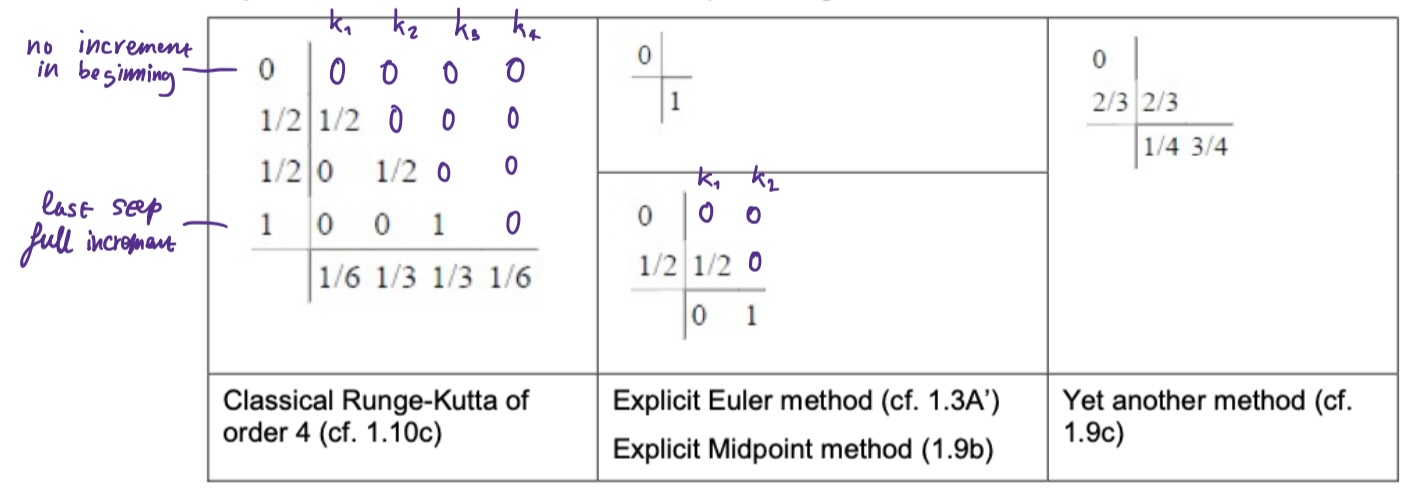
\includegraphics[width=\columnwidth]{images/butcher_tableau}}

\subsection{Adaptive Explicit Runge-Kutta Methods}


        \hrulefill
        \hspace{.5cm}

        \newpage
        \section{Basic Math}

\subsection{Roots}

\begin{align*}
    \sqrt[n]{a}\cdot\sqrt[n]{b} & = \sqrt[n]{a\cdot b} \\
    \frac{\sqrt[n]{a}}{\sqrt[n]{b}} & = \sqrt[n]{\frac{a}{b}} \\
    (\sqrt[n]{a})^m & = \sqrt[n]{a^m} \\
    \sqrt[m]{\sqrt[n]{a}} & = \sqrt[m\cdot n]{a}
\end{align*}

\subsection{Logarithm}

\begin{align*}
    \log_n(a\cdot b) & = \log_n(a) + \log_N(b) \\
    \log_n(a\div b) & = \log_n(a) - \log_N(b) \\
    \log_n(a^b) & = b \cdot \log_n(a)
\end{align*}

\subsection{Trigonometry}

\begin{align*}
    \tan\theta & = \frac{\sin\theta}{\cos\theta} \\
    \sin -\theta & = -\sin\theta\text{ (cos same)} \\
    \sin 2\theta & = 2\sin\theta\cos\theta \\
    \cos 2\theta & = 2\cos^2\theta - \sin^2\theta = 2\cos^2\theta - 1 = 1 - 2\sin^2\theta \\
    \sin(\alpha \pm \beta) & = \sin\alpha\cos\beta\pm\cos\alpha\sin\beta \\
    \cos(\alpha\pm\beta) & = \cos\alpha\cos\beta \mp \sin\alpha\sin\beta
\end{align*}

\subsection{Binomial Coefficient}
\begin{align*}
	\binom{n}{k} = \frac{n!}{k!(n-k)!}
\end{align*}

\subsection{Faculties}
\begin{align*}
    0! = 1, 1! = 1, 2! = 2, 3! = 6, 4! = 24, 5! = 120, 6! = 720
\end{align*}

\subsection{Determinant}
\makebox[\columnwidth]{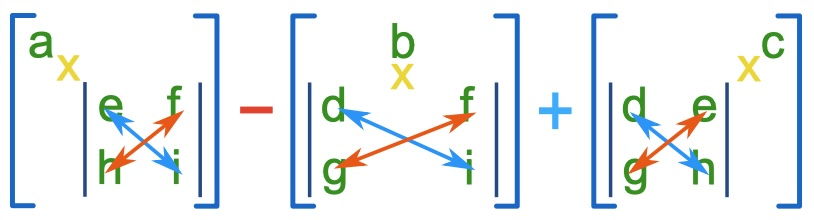
\includegraphics[width=0.5\columnwidth]{images/determinant}}

\begin{align*}
	\det
	\begin{bmatrix}
		a & b \\
		c & d
	\end{bmatrix}
	=
	ad-bc
\end{align*}
\begin{align*}
	\det
	\begin{bmatrix}
		a & b & c \\
		d & e & f \\
		g & h & i
	\end{bmatrix}
	=
	a(ei-fh)-b(di-fg)+c(dh-eg)
\end{align*}

\makebox[\columnwidth]{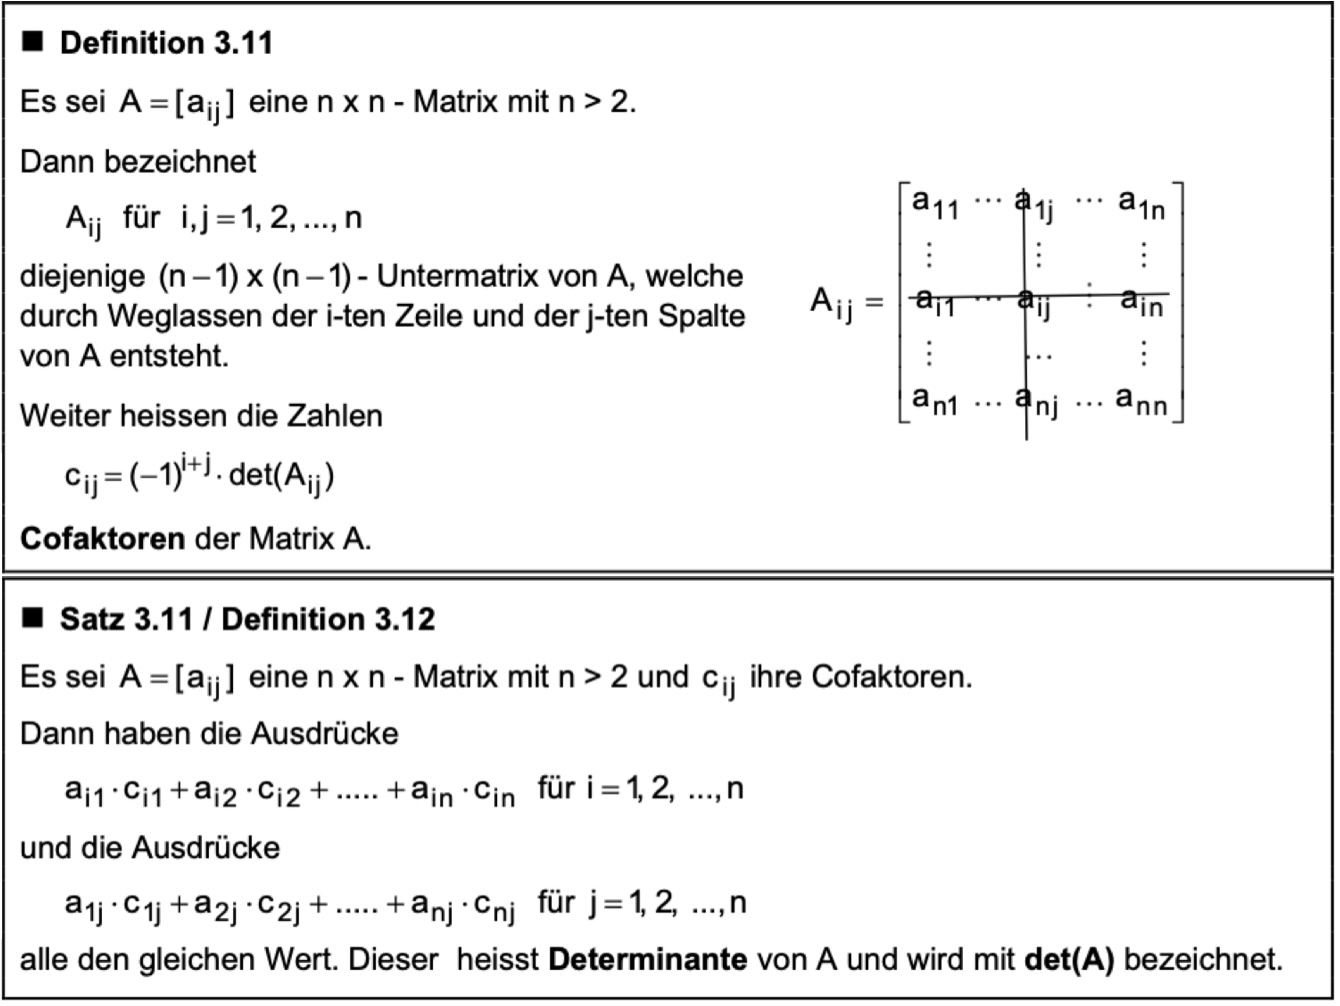
\includegraphics[width=\columnwidth]{images/determinant2}}

\subsubsection{Properties}
\begin{itemize}
	\item $\det\left(A^{-1}\right) = \frac{1}{\det(A)}$
	\item $\det(A^T) = \det(A)$
	\item $\det(I) = 1$
	\item $\det(cA) = c^n\det(A)\quad(\text{for an }n\times n\text{ matrix})$
	\item $\det(AB) = \det(A)\det(B)$
	\item $\det(A) = \prod_{i=1}^n \lambda_i$
\end{itemize}

\subsection{Derivatives}
\begin{tabular}{r|l}
    $f(x)$                & $\frac{df}{dx}$                 \\
    \hline
    $\sinh(x)$            & $\cosh(x)$                      \\
    $\cosh(x)$            & $\sinh(x)$                      \\
    $\mathrm{arcsinh}(x)$ & $1 \div \sqrt{x^2+1}$           \\
    $\mathrm{arccosh}(x)$ & $1 \div \sqrt{x^2 - 1}$ ($1<x$) \\
    $\tan(x)$             & $\cos^{-2}(x)$                  \\
    $\log(x)$             & $x^{-1}$
\end{tabular}

\subsection{Integrals}
\begin{tabular}[h]{rl}
    $\int x^n\ dx$               & $= \frac{1}{n+1}x^{n+1} + C$             \\
    $\int \frac{1}{x}\ dx$       & $= \ln |x| + C$                          \\
    $\int \frac{1}{ax + b}\ dx$  & = $\frac{1}{a} \ln |ax+b| + C$           \\
    $\int \frac{1}{(x+a)^2}\ dx$ & $= -\frac{1}{x+a} + C$                   \\
    $\int \frac{1}{1 + x^2}$     & $= \tan^{-1} x + C$                      \\
    $\int \ln ax\ dx$            & $= x\ln ax - x + C$                      \\
    $\int e^{ax}\ dx$            & $= \frac{1}{a} e^{ax} + C$               \\
    $\int \sin(ax)\ dx$          & $= -\frac{1}{a}\cos(ax) + C$             \\
    $\int \sin^2(ax)\ dx$        & $= \frac{x}{2}-\frac{\sin(2ax)}{4a} + C$ \\
    $\int x\cos x\ dx$           & $= \cos x + x\sin x + C$                 \\
    $\int \sinh(ax)\ dx$         & $= a^{-1}\cosh{ax} + C$                  \\
    $\int \cosh(ax)\ dx$         & $= a^{-1}\sinh{ax} + C$                  \\
\end{tabular}

\subsection{Integration Techniques}

\subsubsection{Integration by Parts}
\begin{equation*}
    \int_a^b u(x)v'(x)\ dx = \left[ u(x)v(x) \right]_a^b-\int_a^bu'(x)v(x)\ dx
\end{equation*}

Or, with $u=u(x)$, $du=u'(x)\ dx$, $v=v(x)$ and $dv=v'(x)\ dx$:
\begin{equation*}
    \int u\ dv=uv - \int v\ du
\end{equation*}

\subsubsection{Substitution}
\begin{equation*}
    \int_a^b f(g(x))\cdot g'(x)\ dx = \int_{g(a)}^{g(b)}f(u)\ du
\end{equation*}

\subsubsection{Leibniz Integral Rule}
\begin{multline*}
    \frac{d}{dx}\left(\int_{a(x)}^{b(x)}f(x,t)\ dt\right)
    =
    \\
    f(x,b(x))\cdot\frac{d}{dx}b(x)
    -f(x,a(x))\cdot\frac{d}{dx}a(x)
    +\int_{a(x)}^{b(x)}\frac{\partial}{\partial x}f(x,t)\ dt
\end{multline*}
Special case where $a(x)=a=\mathrm{const.}$ and $b(x)=b=\mathrm{const.}$:
\begin{equation*}
    \frac{d}{dx}\left(\int_a^b f(x,t)\ dt\right)
    =\int_a^b\frac{\partial}{\partial x}f(x,t)\ dt
\end{equation*}

\subsection{Converting second-order ODEs}

For a second-order equation $y''=f(x,y,y')$, we can introduce $p=y'$, transforming the equation
to $p'=f(x,y,p)$ and thus receiving a system of ODEs with initial conditions
$p(x_0)=y_1, y(x_0) = y_0$.

    \end{multicols}
\end{document}
